\documentclass{standalone}
\usepackage{tikz}
\usetikzlibrary{patterns, positioning}

\begin{document}
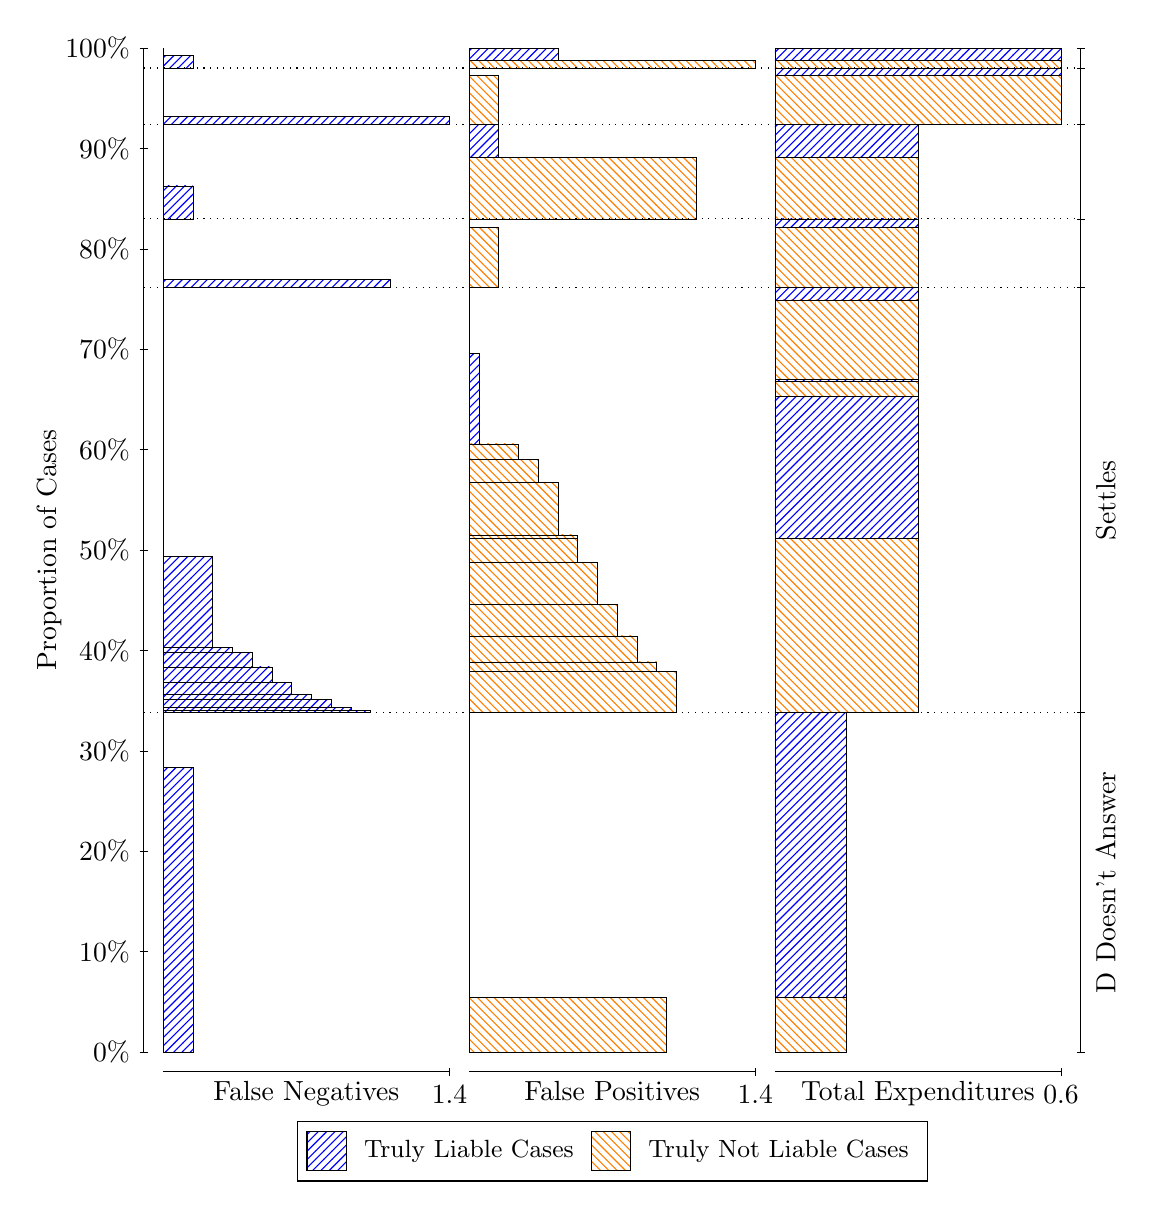
\begin{tikzpicture}
\draw[black, very thin] (1.5,1.75) -- (1.5,14.5);
\node[rotate=90, anchor=center] at (0.3, 8.125) {Proportion of Cases};
\draw[black, very thin] (1.45,1.75) -- (1.55,1.75);
\node[anchor=east] at (1.45, 1.75) {0\%};
\draw[black, very thin] (1.45,3.025) -- (1.55,3.025);
\node[anchor=east] at (1.45, 3.025) {10\%};
\draw[black, very thin] (1.45,4.3) -- (1.55,4.3);
\node[anchor=east] at (1.45, 4.3) {20\%};
\draw[black, very thin] (1.45,5.575) -- (1.55,5.575);
\node[anchor=east] at (1.45, 5.575) {30\%};
\draw[black, very thin] (1.45,6.85) -- (1.55,6.85);
\node[anchor=east] at (1.45, 6.85) {40\%};
\draw[black, very thin] (1.45,8.125) -- (1.55,8.125);
\node[anchor=east] at (1.45, 8.125) {50\%};
\draw[black, very thin] (1.45,9.4) -- (1.55,9.4);
\node[anchor=east] at (1.45, 9.4) {60\%};
\draw[black, very thin] (1.45,10.675) -- (1.55,10.675);
\node[anchor=east] at (1.45, 10.675) {70\%};
\draw[black, very thin] (1.45,11.95) -- (1.55,11.95);
\node[anchor=east] at (1.45, 11.95) {80\%};
\draw[black, very thin] (1.45,13.225) -- (1.55,13.225);
\node[anchor=east] at (1.45, 13.225) {90\%};
\draw[black, very thin] (1.45,14.5) -- (1.55,14.5);
\node[anchor=east] at (1.45, 14.5) {100\%};

\draw[black, very thin] (13.4,1.75) -- (13.4,14.5);
\draw[black, very thin] (13.35,1.75) -- (13.45,1.75);
\node[anchor=west] at (13.35, 1.75) {};
\draw[black, very thin] (13.35,6.0604) -- (13.45,6.0604);
\node[anchor=west] at (13.35, 6.0604) {};
\draw[black, very thin] (13.35,11.456) -- (13.45,11.456);
\node[anchor=west] at (13.35, 11.456) {};
\draw[black, very thin] (13.35,12.33) -- (13.45,12.33);
\node[anchor=west] at (13.35, 12.33) {};
\draw[black, very thin] (13.35,13.533) -- (13.45,13.533);
\node[anchor=west] at (13.35, 13.533) {};
\draw[black, very thin] (13.35,14.246) -- (13.45,14.246);
\node[anchor=west] at (13.35, 14.246) {};
\draw[black, very thin] (13.35,14.5) -- (13.45,14.5);
\node[anchor=west] at (13.35, 14.5) {};

\draw[black, very thin, pattern color=blue, pattern=north east lines] (1.75,1.75) rectangle (2.1259,5.3636);
\draw[black, very thin, pattern color=orange, pattern=north west lines] (1.75,5.3636) rectangle (1.75,6.0604);
\draw[black, very thin, pattern color=blue, pattern=north east lines] (1.75,6.0604) rectangle (4.381,6.0842);
\draw[black, very thin, pattern color=blue, pattern=north east lines] (1.75,6.0842) rectangle (4.1305,6.1254);
\draw[black, very thin, pattern color=blue, pattern=north east lines] (1.75,6.1254) rectangle (3.8799,6.2288);
\draw[black, very thin, pattern color=blue, pattern=north east lines] (1.75,6.2288) rectangle (3.6293,6.2907);
\draw[black, very thin, pattern color=blue, pattern=north east lines] (1.75,6.2907) rectangle (3.3787,6.4447);
\draw[black, very thin, pattern color=blue, pattern=north east lines] (1.75,6.4447) rectangle (3.1282,6.6404);
\draw[black, very thin, pattern color=blue, pattern=north east lines] (1.75,6.6404) rectangle (2.8776,6.8227);
\draw[black, very thin, pattern color=blue, pattern=north east lines] (1.75,6.8227) rectangle (2.627,6.8913);
\draw[black, very thin, pattern color=blue, pattern=north east lines] (1.75,6.8913) rectangle (2.3764,8.0434);
\draw[black, very thin, pattern color=orange, pattern=north west lines] (1.75,8.0434) rectangle (1.75,11.456);
\draw[black, very thin, pattern color=blue, pattern=north east lines] (1.75,11.456) rectangle (4.6316,11.56);
\draw[black, very thin, pattern color=orange, pattern=north west lines] (1.75,11.56) rectangle (1.75,12.33);
\draw[black, very thin, pattern color=blue, pattern=north east lines] (1.75,12.33) rectangle (2.1259,12.749);
\draw[black, very thin, pattern color=orange, pattern=north west lines] (1.75,12.749) rectangle (1.75,13.533);
\draw[black, very thin, pattern color=blue, pattern=north east lines] (1.75,13.533) rectangle (5.3833,13.629);
\draw[black, very thin, pattern color=orange, pattern=north west lines] (1.75,13.629) rectangle (1.75,14.246);
\draw[black, very thin, pattern color=blue, pattern=north east lines] (1.75,14.246) rectangle (2.1259,14.406);
\draw[black, very thin, pattern color=orange, pattern=north west lines] (1.75,14.406) rectangle (1.75,14.5);
\draw[black, very thin, pattern color=orange, pattern=north west lines] (5.6333,1.75) rectangle (8.1391,2.4468);
\draw[black, very thin, pattern color=blue, pattern=north east lines] (5.6333,2.4468) rectangle (5.6333,6.0604);
\draw[black, very thin, pattern color=orange, pattern=north west lines] (5.6333,6.0604) rectangle (8.2644,6.5855);
\draw[black, very thin, pattern color=orange, pattern=north west lines] (5.6333,6.5855) rectangle (8.0138,6.7042);
\draw[black, very thin, pattern color=orange, pattern=north west lines] (5.6333,6.7042) rectangle (7.7632,7.0349);
\draw[black, very thin, pattern color=orange, pattern=north west lines] (5.6333,7.0349) rectangle (7.5126,7.4387);
\draw[black, very thin, pattern color=orange, pattern=north west lines] (5.6333,7.4387) rectangle (7.2621,7.9712);
\draw[black, very thin, pattern color=orange, pattern=north west lines] (5.6333,7.9712) rectangle (7.0115,8.2722);
\draw[black, very thin, pattern color=orange, pattern=north west lines] (5.6333,8.2722) rectangle (7.0115,8.3181);
\draw[black, very thin, pattern color=orange, pattern=north west lines] (5.6333,8.3181) rectangle (6.7609,8.9861);
\draw[black, very thin, pattern color=orange, pattern=north west lines] (5.6333,8.9861) rectangle (6.5103,9.2799);
\draw[black, very thin, pattern color=orange, pattern=north west lines] (5.6333,9.2799) rectangle (6.2598,9.4733);
\draw[black, very thin, pattern color=blue, pattern=north east lines] (5.6333,9.4733) rectangle (5.7586,10.625);
\draw[black, very thin, pattern color=blue, pattern=north east lines] (5.6333,10.625) rectangle (5.6333,11.456);
\draw[black, very thin, pattern color=orange, pattern=north west lines] (5.6333,11.456) rectangle (6.0092,12.227);
\draw[black, very thin, pattern color=blue, pattern=north east lines] (5.6333,12.227) rectangle (5.6333,12.33);
\draw[black, very thin, pattern color=orange, pattern=north west lines] (5.6333,12.33) rectangle (8.5149,13.115);
\draw[black, very thin, pattern color=blue, pattern=north east lines] (5.6333,13.115) rectangle (6.0092,13.533);
\draw[black, very thin, pattern color=orange, pattern=north west lines] (5.6333,13.533) rectangle (6.0092,14.15);
\draw[black, very thin, pattern color=blue, pattern=north east lines] (5.6333,14.15) rectangle (5.6333,14.246);
\draw[black, very thin, pattern color=orange, pattern=north west lines] (5.6333,14.246) rectangle (9.2667,14.34);
\draw[black, very thin, pattern color=blue, pattern=north east lines] (5.6333,14.34) rectangle (6.7609,14.5);
\draw[black, very thin, pattern color=orange, pattern=north west lines] (9.5167,1.75) rectangle (10.425,2.4468);
\draw[black, very thin, pattern color=blue, pattern=north east lines] (9.5167,2.4468) rectangle (10.425,6.0604);
\draw[black, very thin, pattern color=orange, pattern=north west lines] (9.5167,6.0604) rectangle (11.333,8.2722);
\draw[black, very thin, pattern color=blue, pattern=north east lines] (9.5167,8.2722) rectangle (11.333,10.077);
\draw[black, very thin, pattern color=orange, pattern=north west lines] (9.5167,10.077) rectangle (11.333,10.271);
\draw[black, very thin, pattern color=blue, pattern=north east lines] (9.5167,10.271) rectangle (11.333,10.294);
\draw[black, very thin, pattern color=orange, pattern=north west lines] (9.5167,10.294) rectangle (11.333,11.302);
\draw[black, very thin, pattern color=blue, pattern=north east lines] (9.5167,11.302) rectangle (11.333,11.456);
\draw[black, very thin, pattern color=orange, pattern=north west lines] (9.5167,11.456) rectangle (11.333,12.227);
\draw[black, very thin, pattern color=blue, pattern=north east lines] (9.5167,12.227) rectangle (11.333,12.33);
\draw[black, very thin, pattern color=orange, pattern=north west lines] (9.5167,12.33) rectangle (11.333,13.115);
\draw[black, very thin, pattern color=blue, pattern=north east lines] (9.5167,13.115) rectangle (11.333,13.533);
\draw[black, very thin, pattern color=orange, pattern=north west lines] (9.5167,13.533) rectangle (13.15,14.15);
\draw[black, very thin, pattern color=blue, pattern=north east lines] (9.5167,14.15) rectangle (13.15,14.246);
\draw[black, very thin, pattern color=orange, pattern=north west lines] (9.5167,14.246) rectangle (13.15,14.34);
\draw[black, very thin, pattern color=blue, pattern=north east lines] (9.5167,14.34) rectangle (13.15,14.5);
\draw[black, dotted] (1.5,6.0604) -- (13.4,6.0604);
\draw[black, dotted] (1.5,11.456) -- (13.4,11.456);
\draw[black, dotted] (1.5,12.33) -- (13.4,12.33);
\draw[black, dotted] (1.5,13.533) -- (13.4,13.533);
\draw[black, dotted] (1.5,14.246) -- (13.4,14.246);
\draw[black, very thin] (1.75,1.5) -- (5.3833,1.5);
\node[anchor=north] at (3.5667, 1.5) {False Negatives};
\draw[black, very thin] (5.3833,1.45) -- (5.3833,1.55);
\node[anchor=north] at (5.3833, 1.45) {1.4};

\draw[black, very thin] (5.6333,1.5) -- (9.2667,1.5);
\node[anchor=north] at (7.45, 1.5) {False Positives};
\draw[black, very thin] (9.2667,1.45) -- (9.2667,1.55);
\node[anchor=north] at (9.2667, 1.45) {1.4};

\draw[black, very thin] (9.5167,1.5) -- (13.15,1.5);
\node[anchor=north] at (11.333, 1.5) {Total Expenditures};
\draw[black, very thin] (13.15,1.45) -- (13.15,1.55);
\node[anchor=north] at (13.15, 1.45) {0.6};

\node[black, centered, rotate=90] at (13.72, 3.9052) {D Doesn't Answer};
\node[black, centered, rotate=90] at (13.72, 8.7583) {Settles};





\draw (7.449999999999999,1.5) node[draw=none] (baseCoordinate) {};
\begin{scope}[align=center]
        \matrix[scale=0.5, draw=black, below=0.5cm of baseCoordinate, nodes={draw}, column sep=0.1cm]{
            \node[rectangle, draw, minimum width=0.5cm, minimum height=0.5cm, pattern=north east lines, pattern color=blue] {}; &
            \node[draw=none, font=\small] (B) {Truly Liable Cases}; &
            \node[rectangle, draw, minimum width=0.5cm, minimum height=0.5cm, pattern=north west lines, pattern color=orange] {}; &
            \node[draw=none, font=\small] (B) {Truly Not Liable Cases}; \\
            };
\end{scope}

\end{tikzpicture}
\end{document}